
\item A large spherical mass \( M \) is fixed at one position and two identical point masses \( m \) are kept on a line passing through the centre of \( M \) (see figure). The point masses are connected by a rigid massless rod of length \( l \) and this assembly is free to move along the line connecting them. All three masses interact only through their mutual gravitational interaction. When the point mass nearer to \( M \) is at a distance \( r = 3l \) from \( M \), the tension in the rod is zero for \( m = k \left( \frac{M}{288} \right) \). The value of \( k \) is \underline{\hspace{2.5 cm}}.
    \begin{center}
        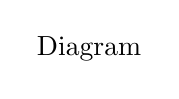
\begin{tikzpicture}
            \node {Diagram};
        \end{tikzpicture}
    \end{center}
